
\section{Introduction}

\begin{frame}
\frametitle{What is ASTRA? - The big picture} 

\begin{columns}

	\begin{column}{8cm}

		\begin{itemize}
		  \item ASTRA: Awareness Services and Systems - Towards Theory and Realization.
		  \item Researching awareness systems and services that are used for social
		  purposes.
		  \item Computer-mediated communication systems that help individuals or groups
		  build and maintain a peripheral awareness of each other.  
		  \item They offer low effort and non-intrusive communication.
		  \item Organizations involved: CTI, Telenor, Philips, NTNU, etc.
		\end{itemize}

	\end{column}

	\begin{column}{5cm}
    
		\begin{figure}
		 	
\includegraphics[scale=0.5]{img/astra_logo.png}
		\end{figure}
    
    \end{column}

\end{columns}


\end{frame}

\begin{frame}
\frametitle{Some key concepts} 

\begin{itemize}
  \item ASTRA Application: transform the services provided by the system
into awareness applications. Two types:
	\begin{itemize}
  		\item \emph{Nimbus}: to make available awareness information to other users.
  		\item \emph{Focus}: to decide what information
			we are interested in and in which way we want to receive it.
	\end{itemize} 

\end{itemize}


 \begin{figure}
 	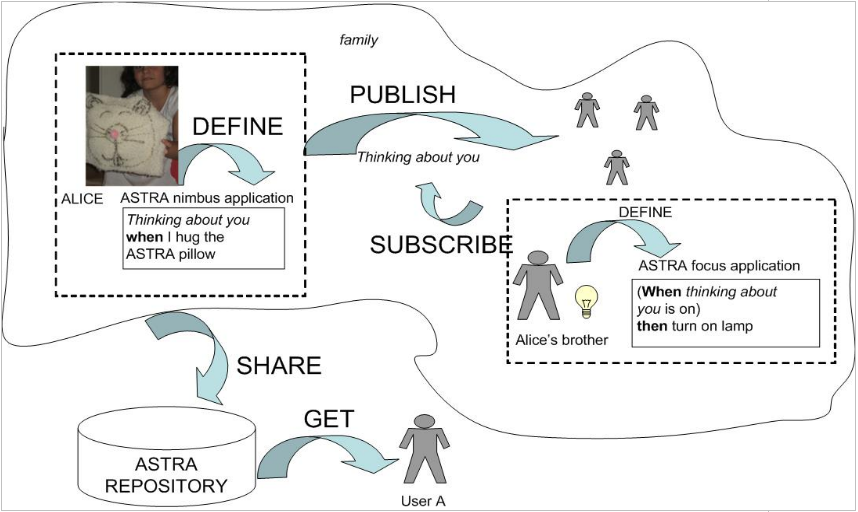
\includegraphics[scale=0.22]{img/astra-applications-schema.png}
 \end{figure}


\end{frame}

\begin{frame}
\frametitle{ASTRA applications example: video} 


 \begin{figure}
 	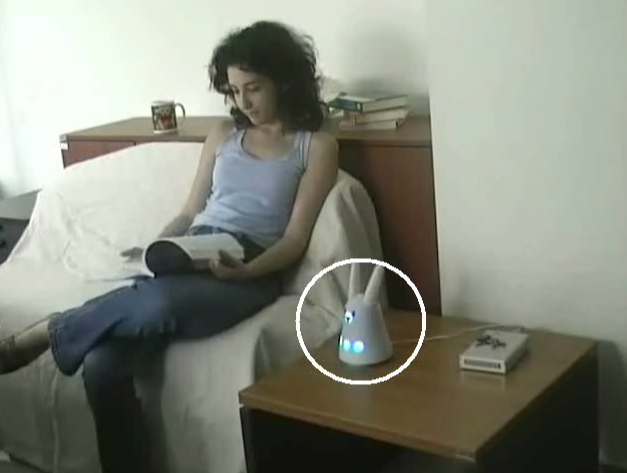
\includegraphics[scale=0.35]{img/video-screenshot.png}
 \end{figure}


\end{frame}

\begin{frame}

\begin{itemize}
  \item Idea: creation and integration of a system to manage the mentioned awareness
applications, including functionalities for sharing, tagging, locating,
appropriating and adapting them.
	\item Taking into account the concerns about privacy in terms of visibility.
\end{itemize}


\begin{figure}
 	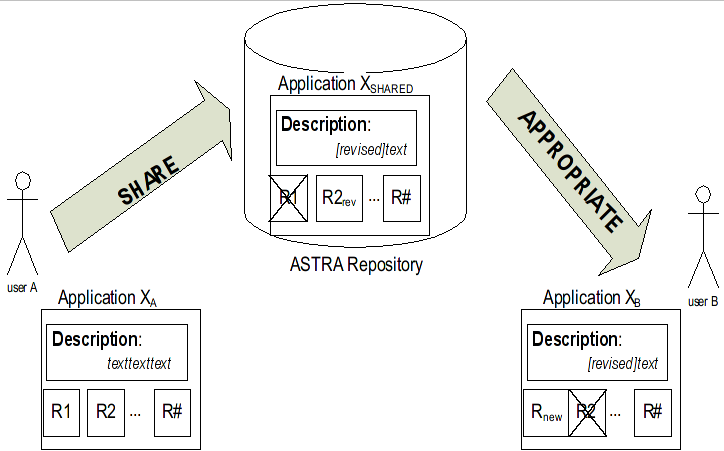
\includegraphics[scale=0.25]{img/repository-appropiation.png}
\end{figure}


\end{frame}
